\chapter{Planteamiento del problema}
El café es un producto altamente consumido en el mundo y es una de las bebidas más populares y preferidas en la sociedad. La producción de café representa un sustento económico para muchas familias en México y más precisamente en Chiapas que es uno de los principales estados exportadores de este grano.

El precio del café tuvo un incremento en el último año, sin embargo, las plagas representan un riesgo para su producción. Algunas plagas como la roya, la araña roja o la broca, pueden causar perdidas severas tanto económicas como de materia prima que bien podrían minimizarse o incluso prevenirse mediante un monitoreo adecuado y regular de la plantación evitando medidas drásticas correctivas como la aplicación de químicos.

El monitoreo de los cultivos de café generalmente require de capacitación o asesoría técnica especializada que muchas veces es cara o inaccesible. El proyecto \textit{Clasificación de hojas de café infectadas por roya usando segmentación por matices en el canal Hue} busca ofrecer una alternativa para quienes apenas ingresan en el mundo del café o bien si no se cuenta con los recursos de inversión suficientes.

\section{Objetivo general}
Demostrar las habilidades adquiridas durante el seminario \textit{Procesamiento Digital de Imágenes: Fundamentos y Aplicaciones con GNU Octave y Open CV} aplicando los principios y técnicas básicas de manera práctica a un proyecto en particular.

\section{Objetivo específico}
Crear un algoritmo que clasifique hojas de café como sanas o infectadas por roya y su nivel de afectación, y evaluar su eficiencia comparando los resultados obtenidos con los proporcionados en el conjunto de datos.

\section{Alcance}
A pesar de que el conjunto de datos de prueba contiene seis clasificaciones para las hojas, el algoritmo desarrollado sólo incluirá la clasificación sana y los cuatro niveles de afectación por roya, excluyendo la clasificación \textit{araña roja} debido a las retricciones en el tiempo del proyecto.

\section{Justificación}
El algoritmo y las técnicas utilizadas pueden aplicarse de manera directa en el mundo real dentro del área de la agricultura y/o agronomía, e idealmente puede servir como base para desarollar procesos automatizados para el control de calidad en el ámbito del café y control de plagas.
 
\section{Especificaciones técnicas}
Se utilizará \textit{Python} como lenguaje de programación para la implementación del algoritmo debido a su facilidad de uso y al amplio número de bibliotecas disponibles para el procesamiento de imágenes tales como \textit{OpenCV}. Así mismo, se utilizará una libreta de \textit{Jupyter} para la ejecución del algoritmo debido a su flexibilidad para ejecutar trozos de código de manera interactiva.

\section{Metodología}
El proceso comienza con la adquisición de las imágenes de las hojas de café, las cuales se transformarán del modelo RGB (Red, Green, Blue) al HSV (Hue, Saturation, Value) para poder aislar el canal Hue. Aplicando diferentes umbrales para los matices, segmentaremos la región de interés en busca de presencia de roya. Usando la imagen segmentada clasificaremos la severidad de la afectación a través de una operación entre el área de la imagen segmentada y una máscara que represente el área de la hoja. Finalmente revisaremos la eficiencia del algoritmo comparando nuestros resultados con las clasificaciones hechas por expertos.

\subsection{Modelo de color HSV}
El modelo de color HSV (Hue, Saturation, Value - Matiz, Saturación, Valor), también conocido como HSB (Hue, Saturation, Brightness - Matiz, Saturación, Brillo) es una representación no-lineal de los colores RGB (Red, Green, Blue - Rojo, Verde, Azul) que ofrece una representación más intuitiva ya que se asemeja a la forma en la que el ojo humano percibe el color.

\begin{figure}[H]
\centering
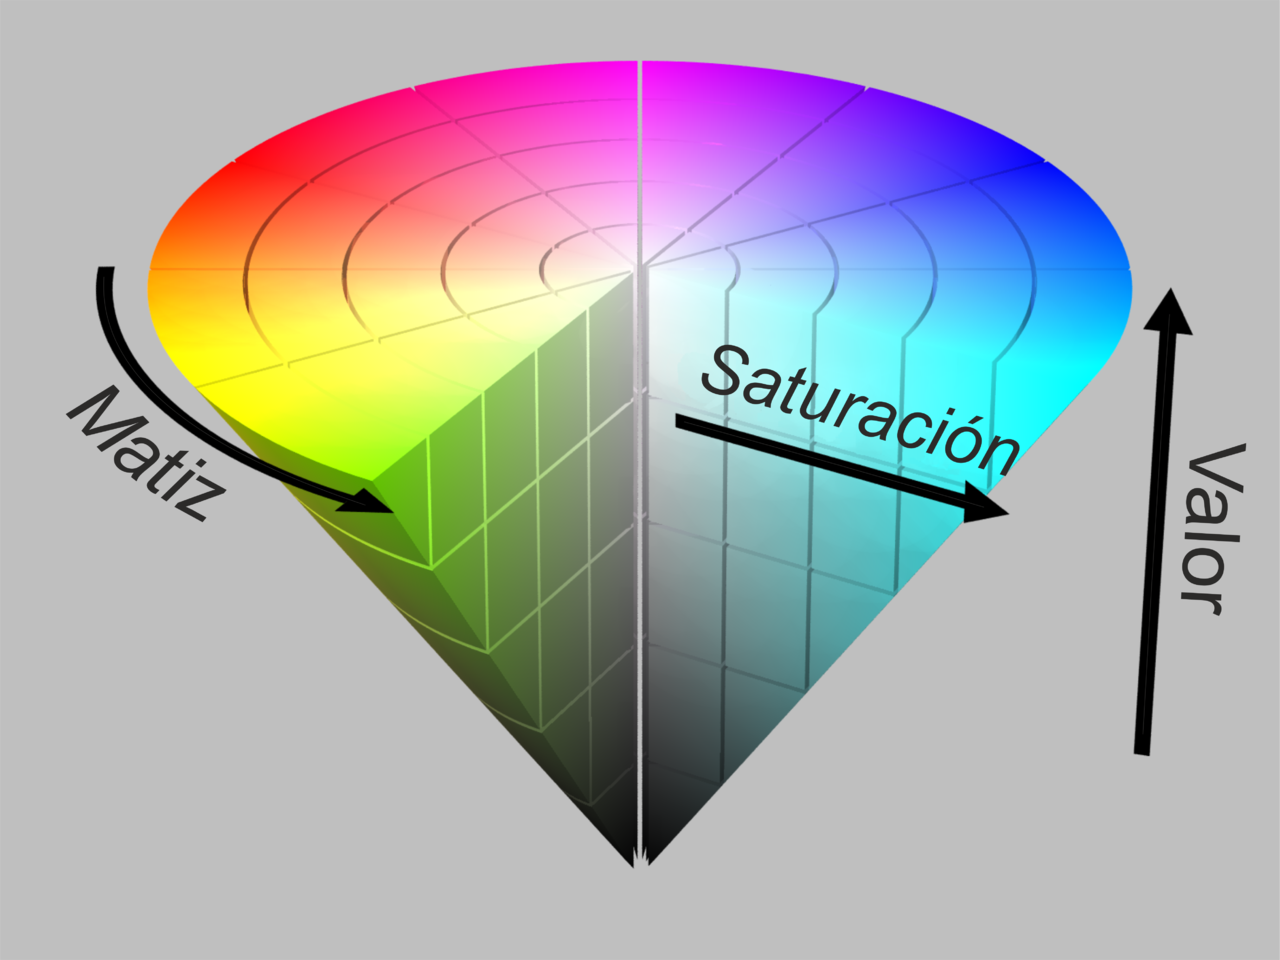
\includegraphics[scale=0.8]{images/hsv_model.png}
\caption{Modelo de color HSV}
\label{img:polygon}
\end{figure}

Una de sus principales ventajas en el ámbito del procesamiento digital de imágenes es que facilita la segmentación de objetos coloridos. Además que, en muchos contextos, el color está asociado a ciertas características inherentes del sistema bajo estudio.

Tal es el caso de la infección por roya en hojas de café, la cual produce cambios de color en las hojas afectadas e incluso cada color indicando un nivel de afectación diferente.

\subsection{RoCoLe: A robusta coffee leaf images dataset}
En el artículo \textit{RoCoLe: A robusta coffee leaf images dataset for evaluation of machine learning based methods in plant diseases recognition} \cite{PARRAGAALAVA2019104414}, Jorge Parraga-Alava, Kevin Cusme, Angélica Loor y Esneider Santander nos proporcionan el dataset \textit{RoCoLe: A robusta coffee leaf images dataset} \cite{RoCoLe} el cual contiene imágenes de hojas de café robusta manualmente clasificadas por su estado de salud y severidad de afectación por roya. Usaremos este dataset como la fuente de imágenes para nuestro proyecto y a su vez nos servirá como referencia para la verificación del desempeño de nuestro algoritmo.

\textit{RoCoLe} continene la información de 390 plantas de café robusta a las cuales se le tomaron 4 muestras de sus hojas haciendo un total de 1560 imágenes. Las muestras fueron tomadas en diferentes condiciones (iluminación, lado de la hoja) para proporcionar un conjunto más diverso de características.

Cada hoja presenta dos clasificaciones: la primera respecto a su estado de salud, ya sea saludable o no-saludable, y la segunda respecto al nivel de afectación por roya en caso de ser una hoja no-saludable. La \Cref{table:rust_levels} presenta la ponderación utilizada para la clasificación de los niveles de afectación.

\begin{table}[H]
\centering
\begin{tabular}{|c|c|c|c|}
\hline 
\textbf{Nivel} & \textbf{Categoría} & \textbf{Descripción} & \textbf{Área afectada} \\
\hline
1 & rust\_level\_1 & Roya nivel 1 & 1 - 5 \% \\
\hline 
2 & rust\_level\_2 & Roya nivel 2 & 6 - 20 \% \\
\hline 
3 & rust\_level\_3 & Roya nivel 3 & 21 - 50 \% \\
\hline 
4 & rust\_level\_4 & Roya nivel 4 & $>$ 50 \% \\
\hline 
\end{tabular}
\caption{Niveles de afectación por roya}
\label{table:rust_levels}
\end{table}